\documentclass[xcolor=table]{beamer}

\usetheme{Boadilla}
% \usetheme{Warsaw}
\usepackage[brazilian]{babel}
\usepackage[utf8]{inputenc}
\usepackage[T1]{fontenc}
\usepackage{color}
%\usepackage{default}
\usepackage{tikz}
%\usetikzlibrary{shapes,arrows}
\usepackage[linesnumbered]{algorithm2e}
\usepackage{multirow}
\usepackage{graphicx}
\usepackage{ragged2e}
\usepackage{outlines}
\usepackage{adjustbox}
\usepackage{tabularx}

\usepackage{hyperref}
\hypersetup{
    colorlinks=true,
    linkcolor=black,
    filecolor=blue,      
    urlcolor=[rgb]{0,0,204},
}


\graphicspath{{imagens/}}



\title{Amazon Web Services (AWS) \\ \vskip 0.2cm Primeiros Passos }
\author{Luan Teylo}
\institute{\textbf{Universidade Federal Fluminense}}

\titlegraphic{
\includegraphics[width=0.2\textwidth]{logo-ic.png}}

\date{Niterói, 06 de Junho 2017}





\setbeamertemplate{navigation symbols}{}
% \makeatletter
\defbeamertemplate*{title page}{mydefault}[1][]
{    

\inserttitlegraphic \usebeamercolor[black]{}\usebeamerfont{title}{}{\insertinstitute}

\vskip 0.5cm

\begin{beamercolorbox}[sep=15pt,center,#1]{title}
      \usebeamerfont{title}\inserttitle%
\end{beamercolorbox}%

\begin{beamercolorbox}[sep=0pt,center,#1]{author}
      \usebeamerfont{author}\insertauthor
\end{beamercolorbox}

\vskip 0.5cm

\begin{beamercolorbox}[sep=15pt,center,#1]{date}
      \small\insertdate
\end{beamercolorbox}

}


\definecolor{LRed}{rgb}{1,.8,.8}
\definecolor{myblue}{RGB}{99,45,247}


\setbeamercolor{footlinecolor}{fg=white,bg=myblue}
\makeatother
\setbeamertemplate{footline}
{
  \setbeamercolor{section in head/foot}{fg=white, bg=black}
  \leavevmode%
  \hbox{%
  
  \begin{beamercolorbox}[wd=0.90\paperwidth,ht=2.25ex,dp=1ex,center]{title in head/foot}%
    \usebeamerfont{title in head/foot} \hskip 1.0cm AWS - Primeiros Passos \hspace*{3em}
    
  \end{beamercolorbox}%
  
  \begin{beamercolorbox}[wd=0.10\paperwidth,ht=2.25ex,dp=1ex,center]{title in head/foot}%
  \insertframenumber{}
  \end{beamercolorbox}}%    
}

\setbeamertemplate{itemize items}[default]



% #####  INICIO ############ %

\begin{document}


{
\setbeamertemplate{footline}{} 
\begin{frame}
   \titlepage
\end{frame}
}

\addtocounter{framenumber}{-1}

% agenda
\begin{frame}{Agenda}
  \tableofcontents
\end{frame}



\section{Página Inicial}
\begin{frame}[c]{Página Inicial}

    \begin{outline}
        \1[]\url{https://aws.amazon.com/pt/}
    \end{outline}
    
    \begin{center}
        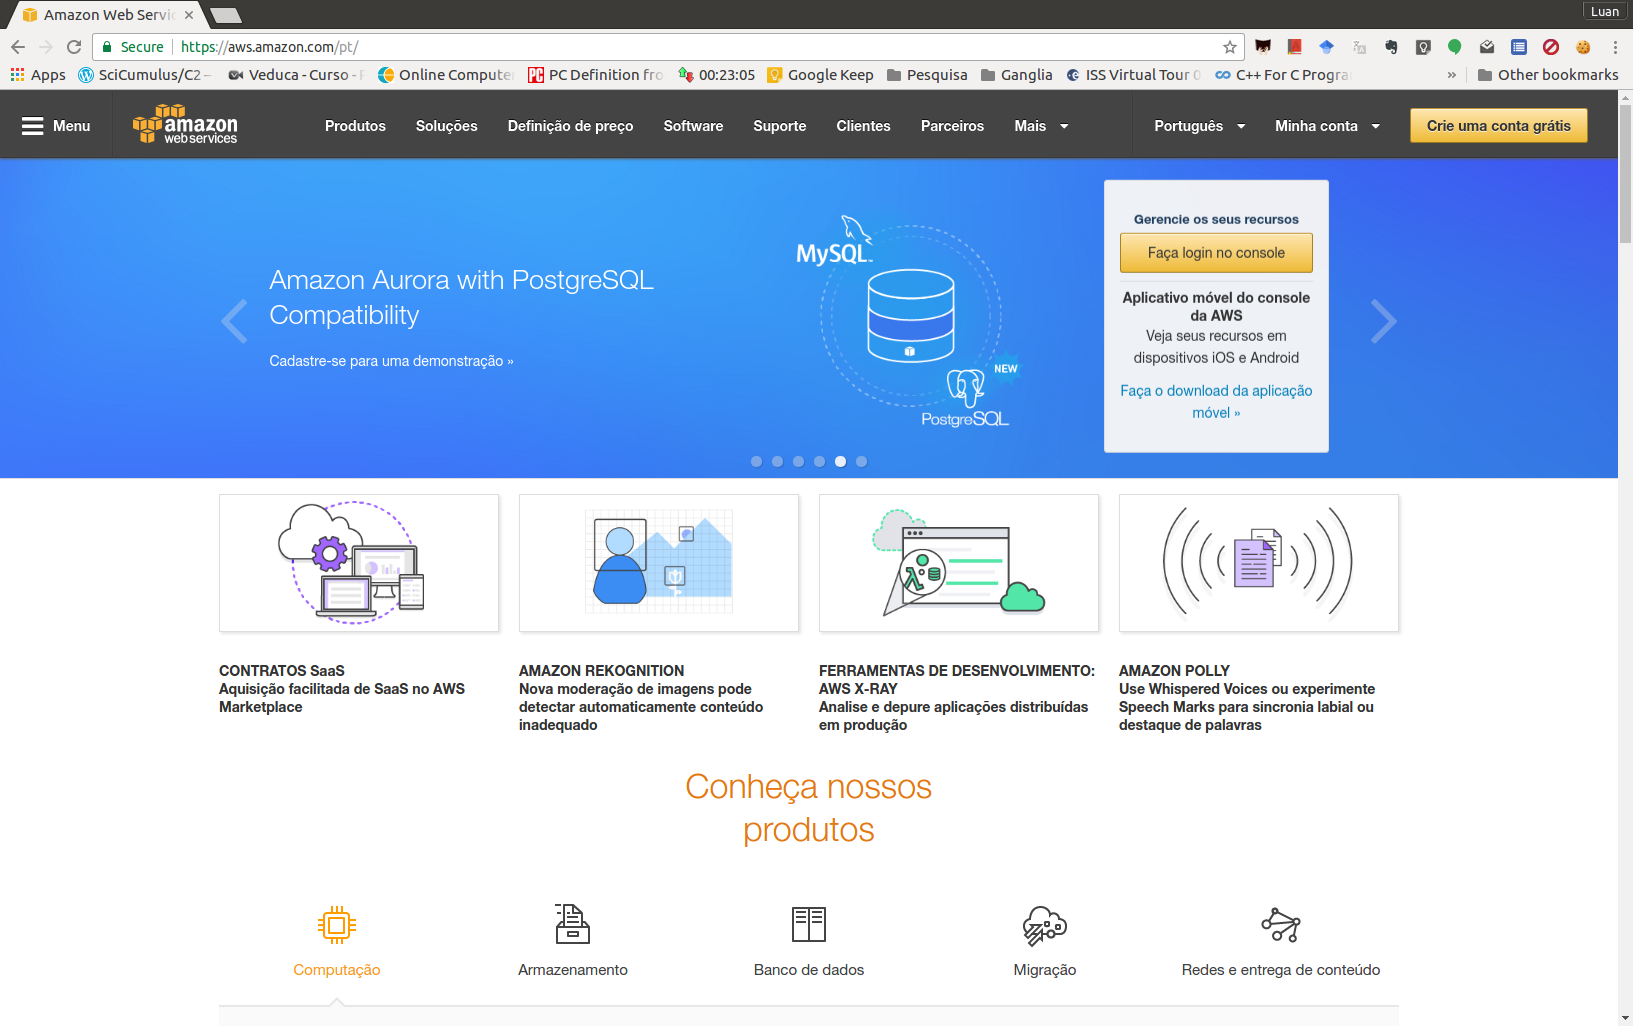
\includegraphics[width=0.75\textwidth]{/tutorial/1_paginaInicial.png} 
    \end{center}
     
    \onslide<2->\begin{outline}
                    \1 É necessário informar cartão de crédito.
                    \1 \alert{Utilize o UFFMail para criar a conta!}
                \end{outline}
\end{frame}




\begin{frame}[c]{AWS  Educate}
    \only<1>{
        \begin{block}{\url{https://aws.amazon.com/pt/education/awseducate/}}
        O AWS Educate é uma iniciativa global da Amazon que disponibiliza a alunos e professores os recursos necessários para acelerar esforços de aprendizado relacionados à nuvem.
        \end{block}
    }
    \only<2>{
        \begin{center}
            
\includegraphics[width=0.4\textwidth]{/tutorial/2_aws_educate_aluno.png} 
        \end{center}
    }
    \only<3>{
        \begin{center}
            Vídeo 1: \href{run:./1_aws_educate.ogv}{Inscrição no AWS Education}
        \end{center}
    }
\end{frame}



\section{AWS Console}
\begin{frame}[c]{Console}

    \only<1>{
        \begin{outline}
            \1[]\url{https://console.aws.amazon.com/}
        \end{outline}
        
        \begin{center}
            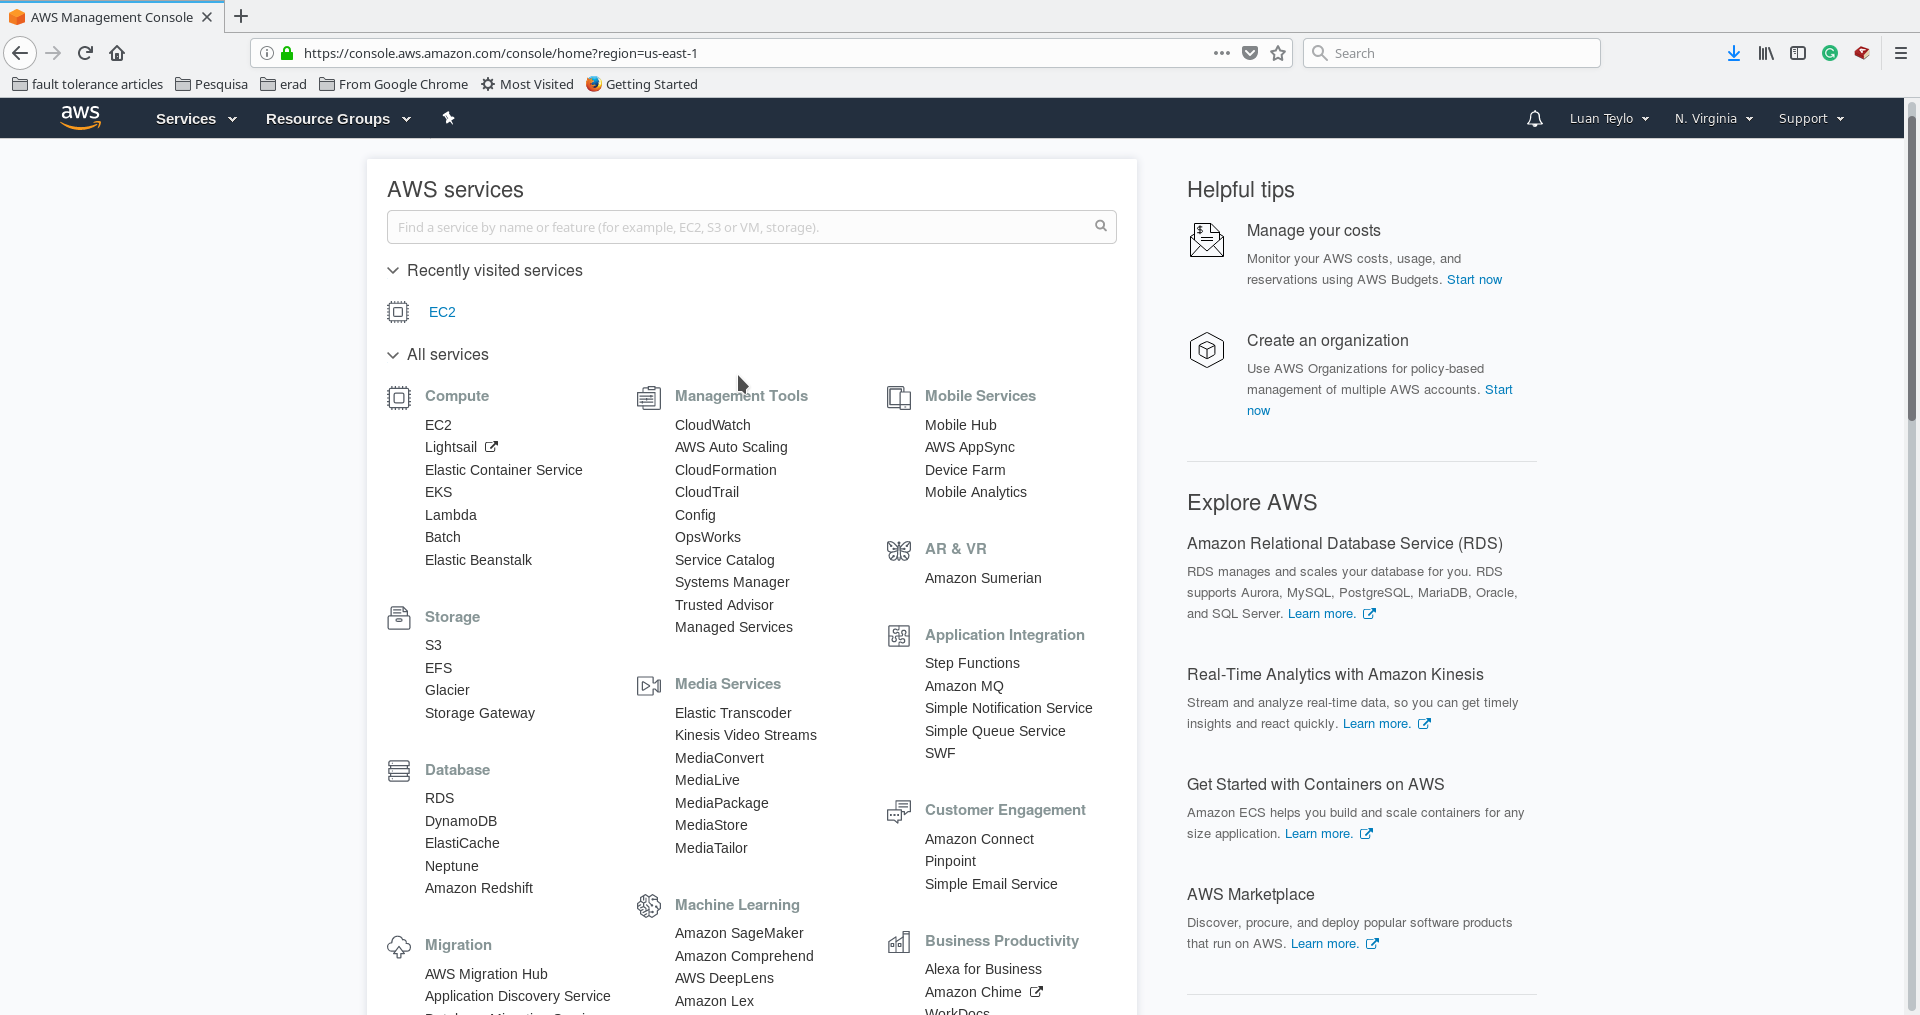
\includegraphics[width=0.75\textwidth]{/tutorial/console.png} 
        \end{center}
    }
    
    \only<2>{
        \begin{outline}
            \1 Billing & Cost Management Dashboard
            \1 Elastic Compute Cloud (EC2)
            \1 Amazon Simple Storage Service (Amazon S3)
        \end{outline}
    }
    
\end{frame}


\section{Management DashBoard}
\begin{frame}[c]{Console}{Management DashBoard}

        \begin{outline}
            \1[]\url{https://console.aws.amazon.com/billing/}
        \end{outline}
        
        \begin{center}
            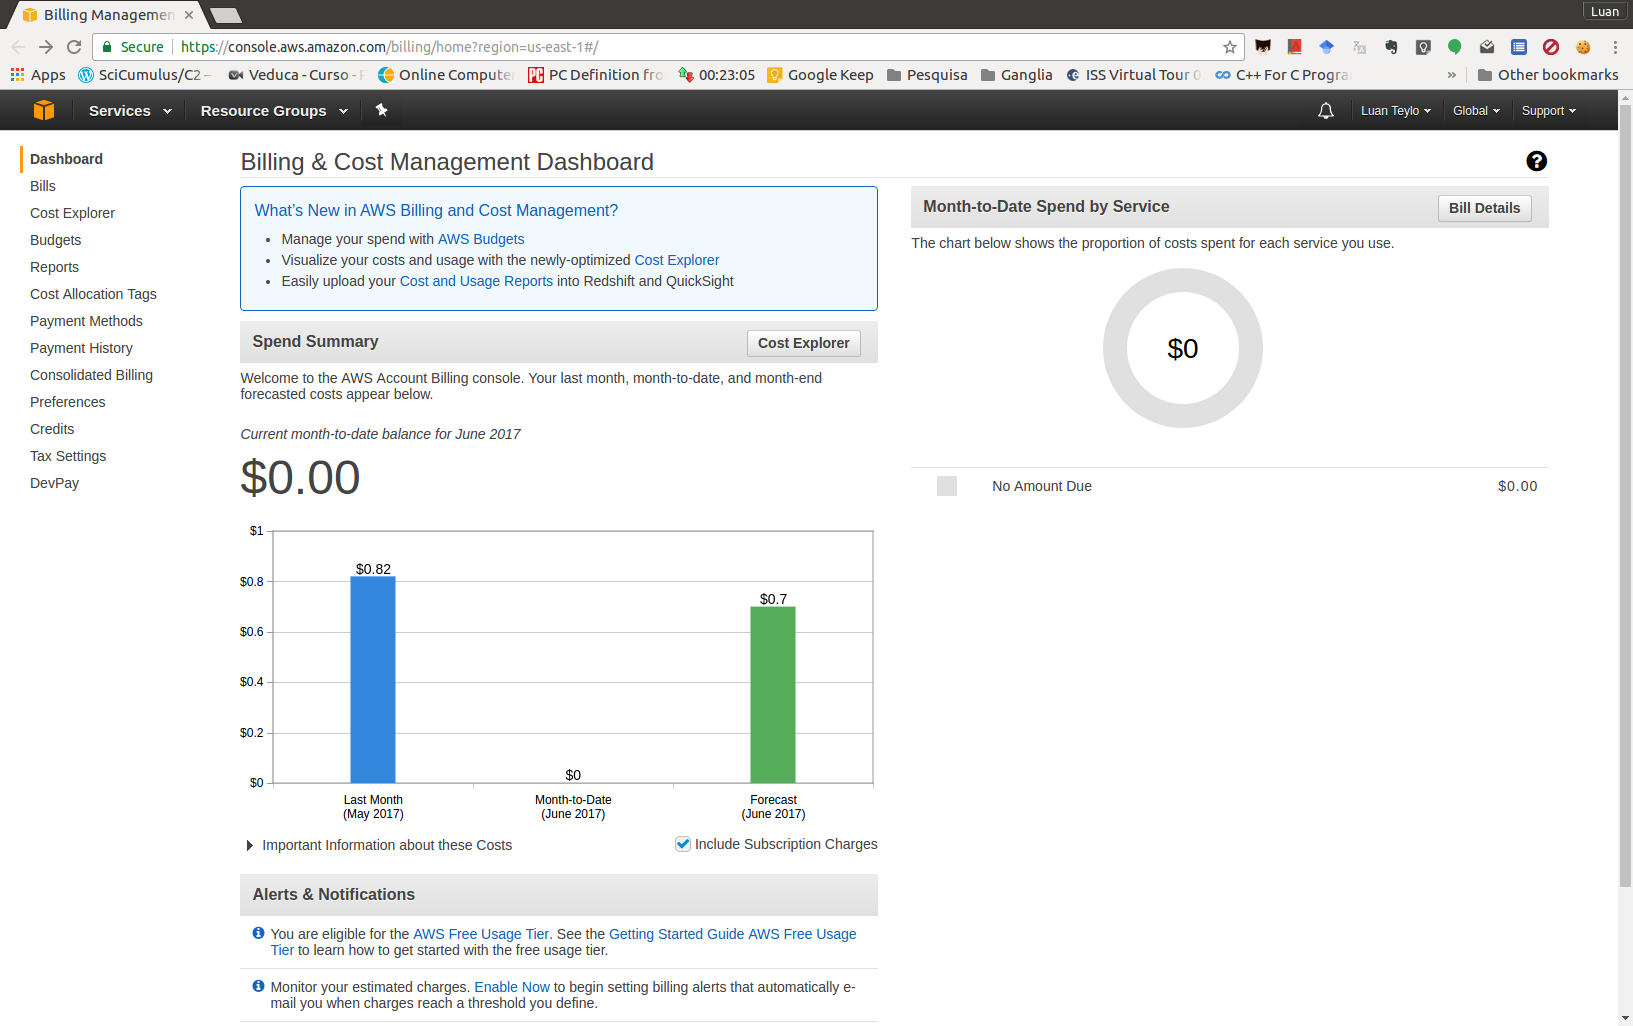
\includegraphics[width=0.75\textwidth]{/tutorial/managementDashboard.png} 
        \end{center}

\end{frame}


\section{Elastic Computer Cloud (EC2)}
\begin{frame}[c]{Elastic Computer Cloud}{EC2}

        \begin{outline}
            \1[]\url{https://console.aws.amazon.com/ec2/}
        \end{outline}
        
        \begin{center}
            \begin{outline}                
                \1 Disponibiliza capacidade computacional segura e redimensionável na nuvem.
                \1 A interface de serviço da Web do Amazon EC2 permite que você obtenha e configure o ambiente facilmente. 
                \1 Oferece um controle completo de seus recursos computacionais.
            \end{outline}
        \end{center}

\end{frame}


\begin{frame}[c]{EC2}{Tipos de Instâncias}


        \begin{outline}
            \1[]\url{https://aws.amazon.com/pt/ec2/instance-types/}
        \end{outline}
        
      
            \begin{outline}          
            \only<1-2>{\1[] T2 - Instância de uso geral de custo mais baixo}
            \only<3>{\1[] C4 - Instâncias otimizadas para computação}
            \begin{figure}
                \only<1-2>{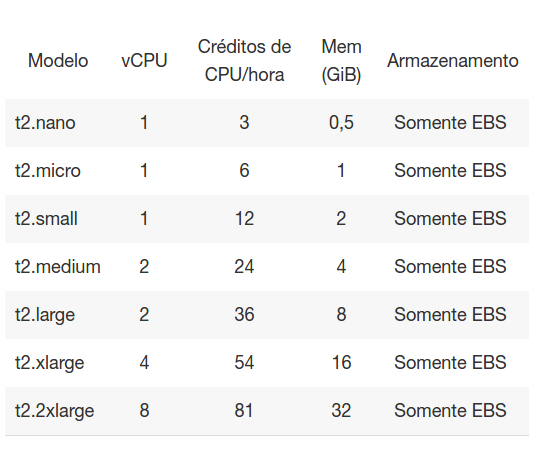
\includegraphics[width=0.4\textwidth]{/tutorial/tipo_t2.png}}
                \only<3>{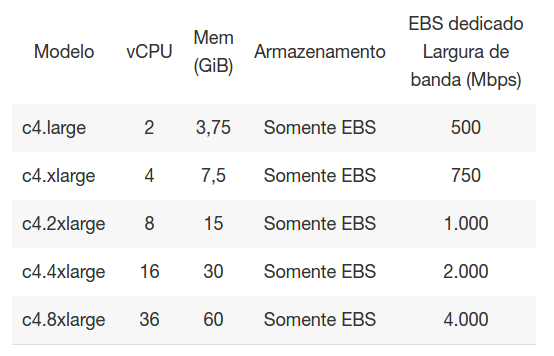
\includegraphics[width=0.4\textwidth]{/tutorial/tipo_c4.png}}
                \hfill
                \only<1>{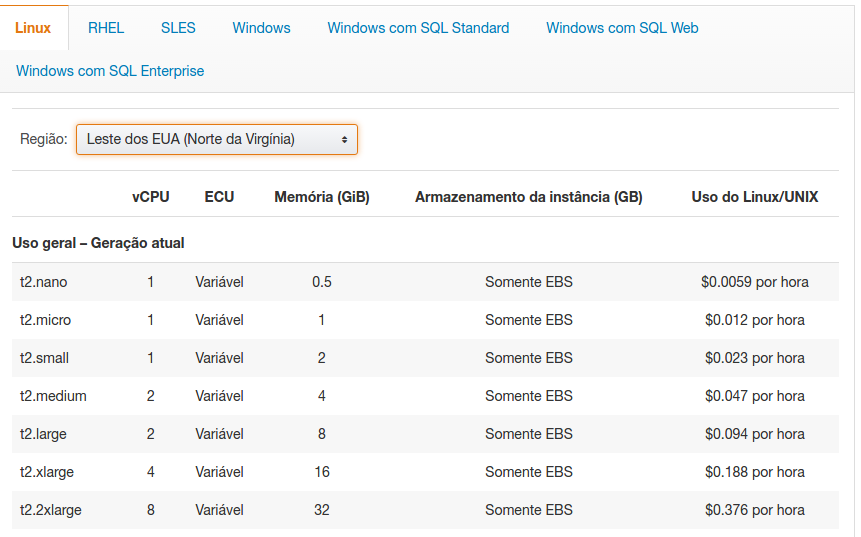
\includegraphics[width=0.4\textwidth]{/tutorial/preco_1.png}}
                \only<2>{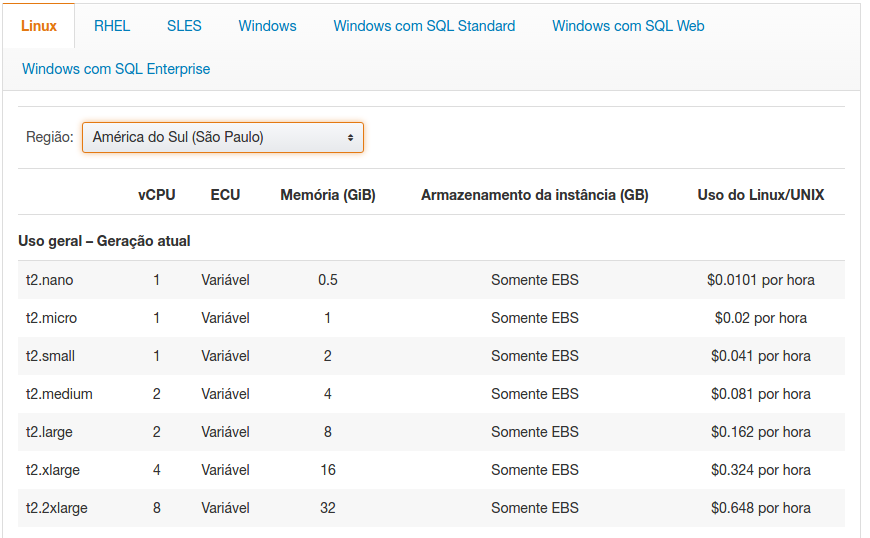
\includegraphics[width=0.4\textwidth]{/tutorial/preco_2.png}}                
                \only<3>{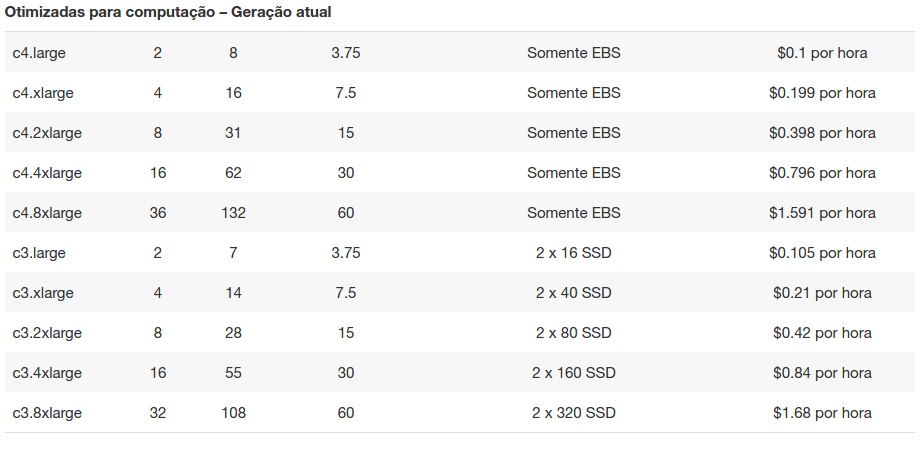
\includegraphics[width=0.4\textwidth]{/tutorial/preco_3.png}}
            \end{figure}
            
            
            \end{outline}
       
\end{frame}


\begin{frame}[c]{EC2}{Conceitos Básicos}

        \begin{outline}
            \1[]\url{https://console.aws.amazon.com/ec2/}
        \end{outline}
        
        
        \begin{center}
            \begin{outline}                
               \1[] \textbf{Etapa 1:} Inicie as instâncias
               \1[] \textbf{Etapa 2:} Conecte-se 
               \1[] \textbf{Etapa 3:} Utilize
               \1[] \textbf{Etapa 4:} Encerre/\alert{delete} as instâncias
            \end{outline}
        \end{center}

\end{frame}


\begin{frame}[c]{EC2} {Iniciando as Instâncias}

        \begin{center}
            Vídeo 2: \href{run:./2_running.ogv}{Etapa 1: Iniciando as instâncias}
        \end{center}  

\end{frame}



\begin{frame}[c]{EC2}{Conectando}
        \begin{center}
            \begin{outline}                
                \1 Iremos utilizar um cliente SSH instalado na máquina local.
                \1 Atenção! Em um AMI padrão apenas a porta 22 está habilitada para receber conexão SSH.
            \end{outline}
        \end{center}
        \begin{center}
        
            \textit{/etc/ssh/sshd\_conf}
            
            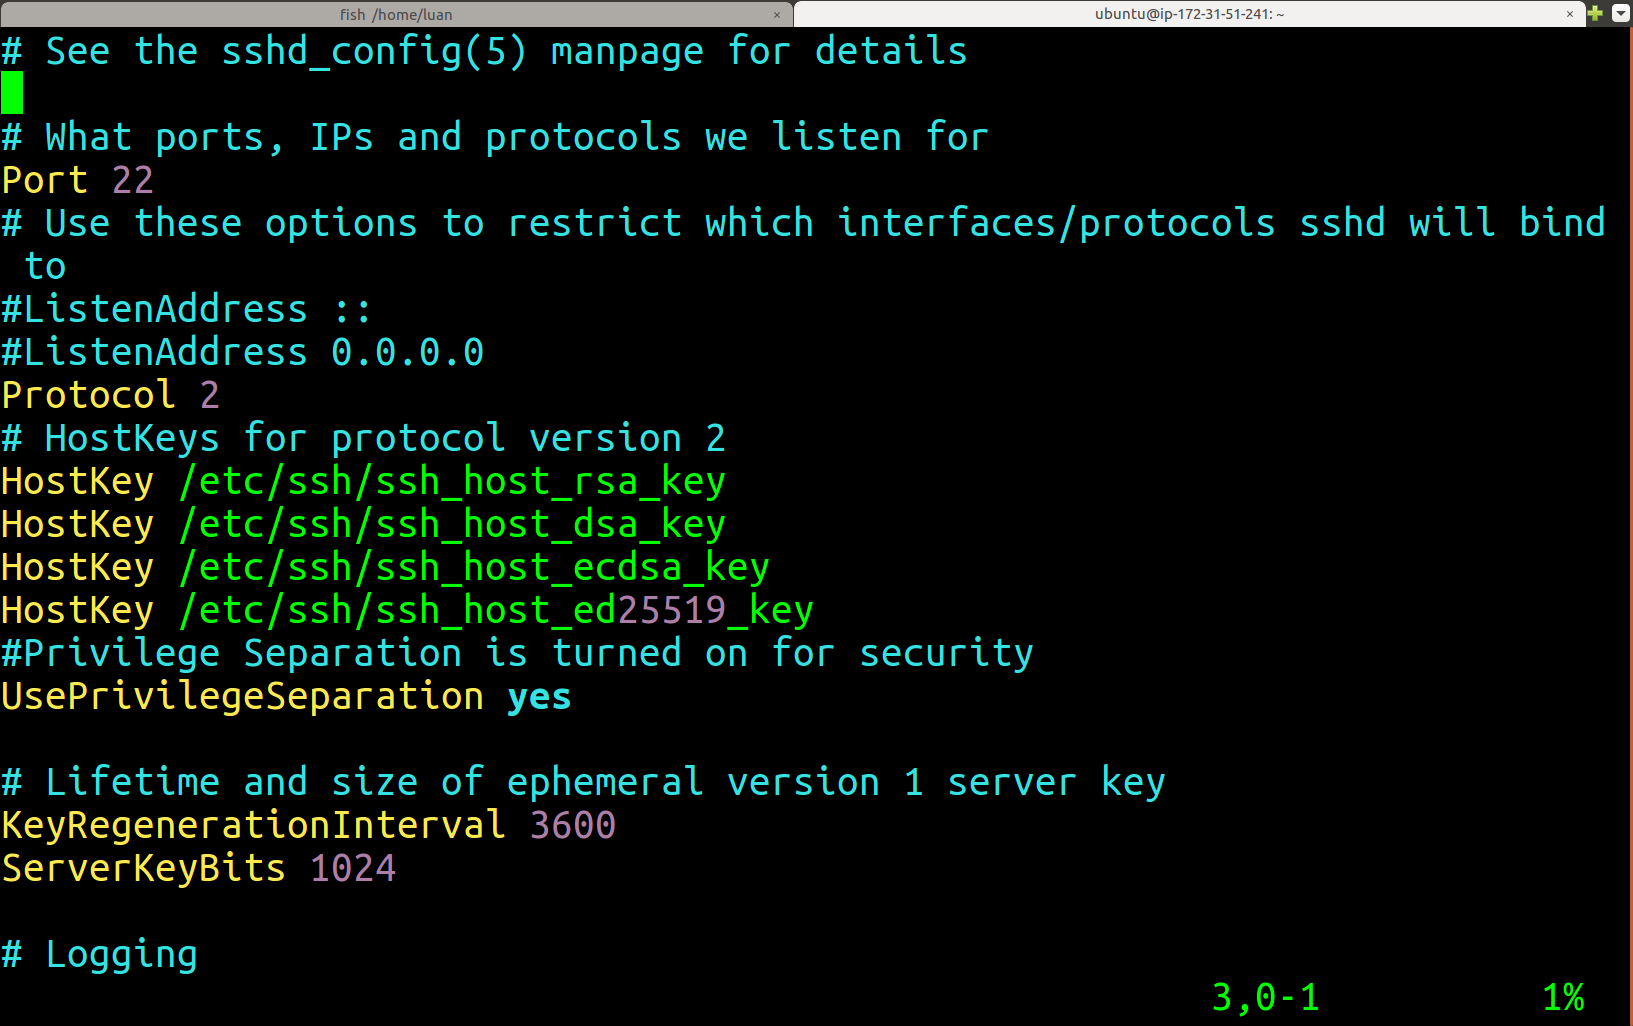
\includegraphics[width=0.7\textwidth]{/tutorial/sshd_conf.png}
        \end{center}

\end{frame}


\begin{frame}[c]{EC2}{Conectando}

        \begin{center}
            Vídeo 3: \href{run:./3_connecting.ogv}{Etapa 2: Conectando-se}
        \end{center}
      
\end{frame}



\begin{frame}[c]{EC2}{Utilizando}


        \begin{center}
            

            \begin{outline}
            \1[] Dica:
            \2[] Utilize o SCP para transferir dados/programas para a VM 
            \2[] 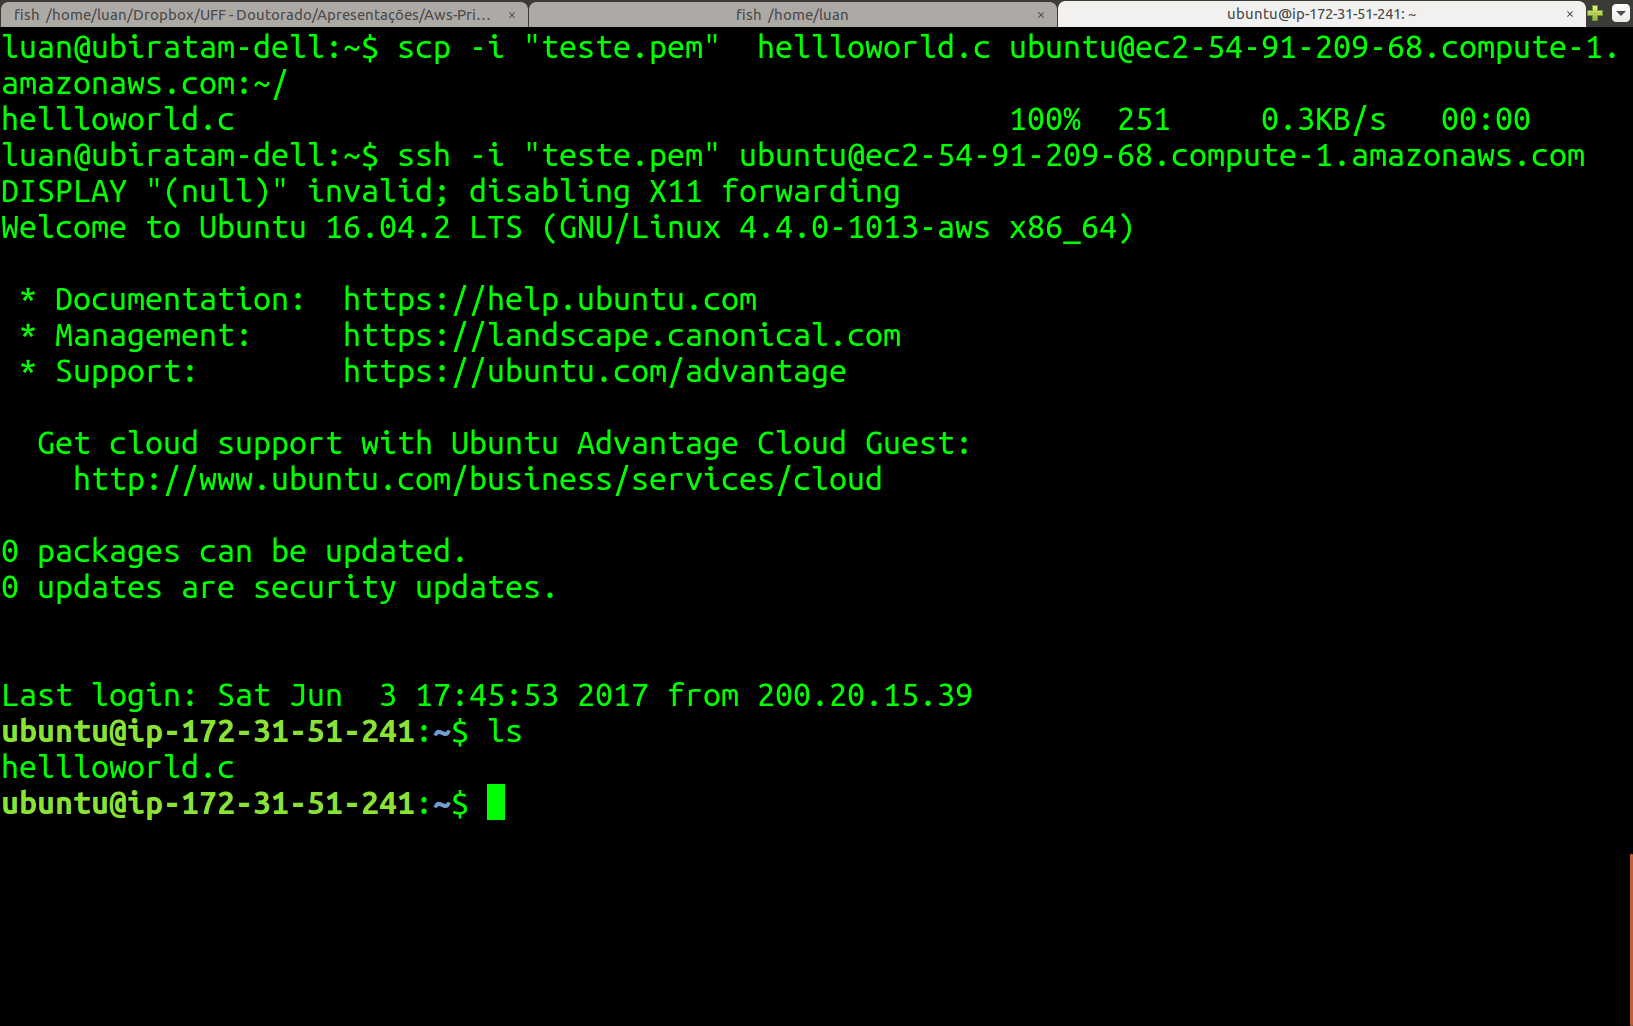
\includegraphics[width=0.7\textwidth]{/tutorial/scp.png}
            
            \end{outline}
        \end{center}      
\end{frame}


\begin{frame}[c]{EC2}{Deletando}

        \begin{center}
            Vídeo 4: \href{run:./4_encerrando.ogv}{Etapa 3: deletando}
        \end{center}
      
\end{frame}




\section{Simple Storage Service (S3)}
\begin{frame}[c]{Simple Storage Service (S3)}

        \begin{outline}
            \1[]\url{https://console.aws.amazon.com/s3/}
        \end{outline}
        
        \begin{center}
            \begin{outline}                
                \1 É um serviço de armazenamento de objetos
                \1 Foi projetado para oferecer uma durabilidade de 99,999999999\% e escalar mais de 1 trilhão de objetos em todo o mundo.
                \vskip 0.5cm
                \2[] Serviços como Spotify, Github, Quora e Sharelatex utilizam o S3.
            \end{outline}
        \end{center}  
        
\end{frame}


\begin{frame}[c]{S3}{Política de Cobrança}


        \begin{outline}
            \1[]\url{https://aws.amazon.com/pt/s3/pricing/}
        \end{outline}
        
            
            \begin{center}
                \only<1>{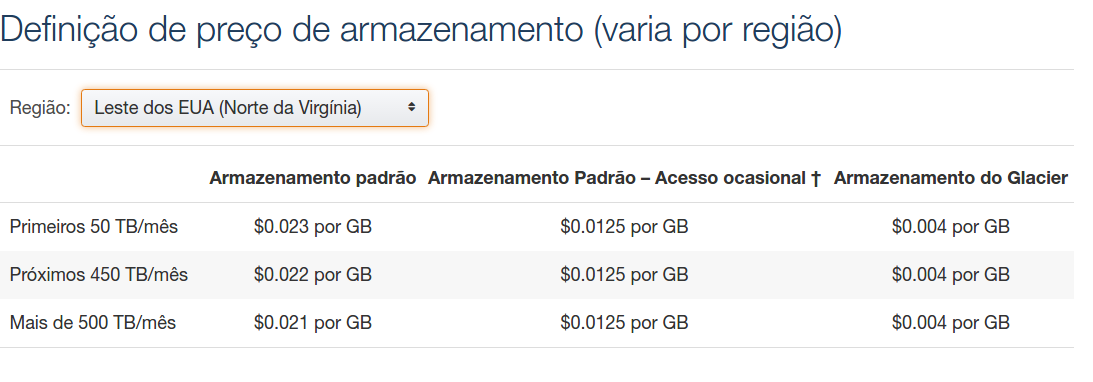
\includegraphics[width=0.75\textwidth]{/tutorial/s3_precos.png}}
                \only<2>{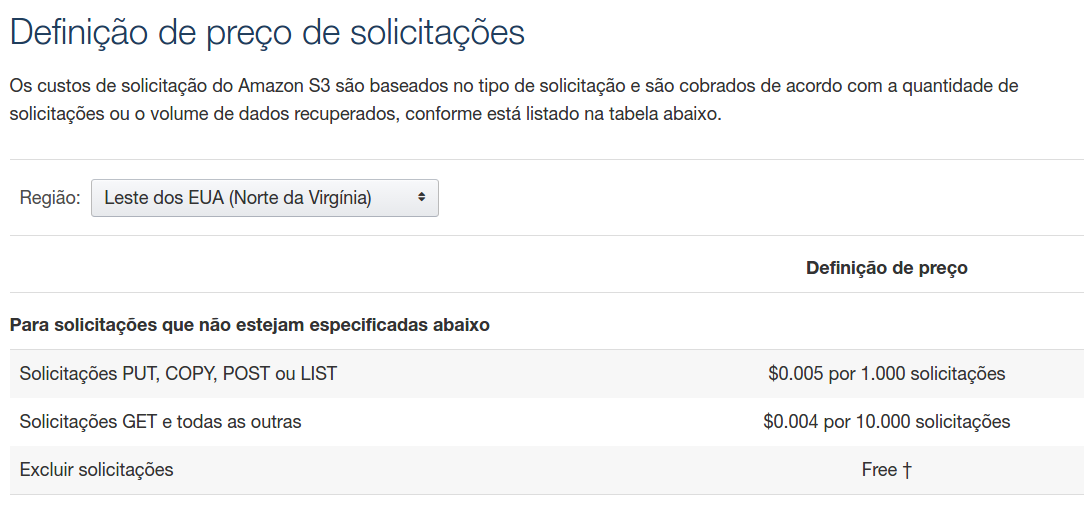
\includegraphics[width=0.75\textwidth]{/tutorial/s3_preco2.png}}
                
            \end{center}           
       
\end{frame}


\begin{frame}[c]{S3}{Utilizando o S3}

        
        \begin{center}
            Vídeo 5: \href{run:./5_s3.ogv}{Criando um Bucket no S3}
        \end{center}       
       
        
            \begin{outline}
                \1 Para criar um ponto de montagem do S3 utilizaremos o s3fs
                \2 Disponível em: \url{https://github.com/s3fs-fuse/s3fs-fuse}
            \end{outline}
        
        \begin{center}
            Vídeo 6: \href{run:./6_mountS3.ogv}{Utilizando o S3 em uma instância EC2}
        \end{center}       
       
\end{frame}

{
\setbeamertemplate{footline}{} 
\begin{frame}[c]{}

    \begin{center}

 
            Dúvidas ?
            \vskip 0.5cm
            %  Favor Manter os créditos do autor%
            Todo os arquivos desta apresentação foram disponibilizados inicialmente em: \url{https://github.com/luanteylo/Tutorial-AWS}
             
      
         
    \end{center}
     
       
\end{frame}
}



\end{document}




